% Workshop paper draft, ACM sigconf. Build: latexmk -pdf main.tex
\documentclass[sigconf,nonacm]{acmart}
\settopmatter{printacmref=false}
\setcopyright{none}
\renewcommand\footnotetextcopyrightpermission[1]{}
\usepackage{booktabs}

\begin{document}

\title{Catch Leaks at Commit Time: Dataset Versioning\\with Built-in Split Hygiene}

\author{Raj Alamuri}
\affiliation{\institution{Independent researcher}\city{London}\country{United Kingdom}}
\email{rajanalamuri@gmail.com}

\begin{abstract}
Train/test leakage keeps resurfacing in published benchmarks, yet the tools teams use to version
datasets record \emph{what} the data is, not whether its splits are sound. We argue that split
hygiene belongs in the same step that fingerprints a dataset: a commit that writes an immutable
manifest should also refuse, or loudly flag, leaky splits. We present \textsc{mlfingerprint}, an
open-source library that versions datasets of any modality on any object store as a manifest of
content hashes, and at commit time keeps recordings and frame sequences together, detects
augmented copies, exact and near-duplicate files, repeated text records, temporal overlap and
leaks from a parent dataset's evaluation split. On MNIST, Fashion-MNIST and the 122k-file COCO 2017
annotation set every reported count matches independently computed ground truth; a full commit
costs 23--35\,s on two vCPUs and an unchanged re-commit 7--23\,s. Its 64-bit perceptual check,
run on CIFAR-10, flags 91 test images with a near-duplicate in the training set; 63 are in the
ciFAIR list, and our review finds 24 of the remaining 28 are also duplicates that ciFAIR-10 still
contains. Recall against ciFAIR is low (22\%), which we report as the price of a check cheap
enough to run on every commit.
\end{abstract}

\begin{CCSXML}
<ccs2012>
<concept><concept_id>10002951.10002952.10003219</concept_id><concept_desc>Information systems~Information integration</concept_desc><concept_significance>300</concept_significance></concept>
<concept><concept_id>10010147.10010257</concept_id><concept_desc>Computing methodologies~Machine learning</concept_desc><concept_significance>500</concept_significance></concept>
</ccs2012>
\end{CCSXML}
\ccsdesc[300]{Information systems~Information integration}
\ccsdesc[500]{Computing methodologies~Machine learning}

\keywords{dataset versioning, data leakage, reproducibility, near-duplicates, MLOps}
\maketitle

\section{Introduction}
Leakage between training and evaluation data inflates reported performance. A survey of
ML-based science found leakage in 294 papers across 17 fields \cite{kapoor2023leakage};
duplicates and near-duplicates sit in the test sets of CIFAR \cite{barz2020cifair},
ImageNet \cite{kisel2024flaws} and other visual benchmarks \cite{ramos2025leakage}; and
sensor and time-series work routinely splits windows of the same recording or subject across
train and test \cite{roberts2017cv}. These problems are usually found long after a dataset is
published, by an audit.

Meanwhile most teams already run a step that touches every file before training: dataset
versioning \cite{dvc,lakefs,armbrust2020delta}. Versioning tools hash files to make runs
reproducible, but they treat the train/val/test assignment as opaque. Leakage checkers exist,
but as separate, after-the-fact tools, mostly for single data frames \cite{deepchecks,mlleak,leaklens}.
Our thesis is simple: \emph{the commit that fingerprints a dataset already has the content hash,
the path, the split and the lineage of every file, which is exactly what most leakage checks
need}. Running them there costs little and puts the result in the manifest that the training
run pins.

\textbf{Contributions.} (1) A manifest-based dataset versioning design where split hygiene is part
of the commit (\S\ref{sec:design}); (2) group-aware automatic splitting and checks that work across
images, audio, video frames, sensor streams, text and tables on local disk, S3, Azure Blob, GCS and
Databricks volumes; (3) an evaluation against independent ground truth on four public datasets,
including a reproduction of the ciFAIR near-duplicate audit that surfaces duplicates its list
misses (\S\ref{sec:eval}). The library is MIT-licensed \cite{mlfingerprint}.

\section{Design}\label{sec:design}
\textbf{Version the description, not the data.} A version is an immutable folder holding an
\texttt{index.jsonl.gz} (one row per file: path, split, label, size, SHA-256, modality, optional probe
metadata), per-split file lists and a \texttt{manifest.json} written last, which makes the commit
atomic on object stores. The dataset fingerprint is a digest over \texttt{(path|split, sha256)}, so
moving one file between splits changes it. Files can be referenced in place (zero copy, with
\texttt{verify} detecting drift), copied, hard-linked or stored content-addressed so identical files
are kept once across versions. A SQLite cache keyed by \texttt{(uri, size, stamp)}, where the stamp is
\texttt{mtime\_ns:ctime\_ns:inode} locally and the ETag remotely, means an unchanged re-commit hashes
nothing. Versions get semantic numbers derived from the diff (new modality: major; added files: minor;
removed or modified: patch) and can be tagged and checked out.

\textbf{Splits that respect groups.} When no split is given, existing \texttt{train/}, \texttt{val/},
\texttt{test/} folders or names such as \texttt{train2017} are used; otherwise files are assigned by a
stable hash of a \emph{group key}, so the assignment never changes as data is added. The default
key keeps together what must not be separated: a recording or session folder, a frame sequence
(detected only if numbering is dense or regular, so sparse image ids are not mistaken for frames),
an image and its label file, and an augmented copy and its original. Temporal splits by ratio or
cutoff put the oldest recordings in train; row-level cutoffs inside one long series are stored in
the manifest.

\textbf{Checks at commit time.} Each commit records a \texttt{quality} block and warnings:
\emph{augmentation leaks} (copies such as \texttt{img\_7\_hflip.png} or files under \texttt{aug/} in a
different split than their original, or in val/test); \emph{exact duplicates} across splits (equal
SHA-256); \emph{record overlap} for text and tables (normalised line hashes shared between train and
val/test); \emph{temporal overlap}; \emph{parent leaks}, where a derived dataset's training files are
copies or augmentations of a parent version's val/test files; and \emph{split drift} between versions.
Augmentation leaks can be made fatal for CI.

\textbf{Near-duplicates.} Optionally, each image gets a 64-bit difference hash (dHash)
\cite{krawetz2013dhash}, cached by its SHA-256. To find all cross-split pairs within Hamming distance
$T$, each hash is cut into $T{+}1$ disjoint chunks; by the pigeonhole principle, two hashes within
distance $T$ agree on at least one chunk, so only items sharing a chunk value are compared. The
search is exact, a simple case of multi-index hashing \cite{norouzi2012mih}.

\textbf{Storage and safety.} Storage goes through \texttt{fsspec}; integration tests run against S3,
Azure and GCS emulators. Paths in an index are validated before checkout, a tampered index is refused,
credentials are never written to manifests, and loaders never unpickle data.

\section{Evaluation}\label{sec:eval}
All runs used two vCPUs on local disk. Ground truth was computed from the raw dataset files without
\textsc{mlfingerprint}.

\textbf{Correctness and cost.} On MNIST \cite{lecun1998mnist} and Fashion-MNIST \cite{xiao2017fashion}
(70,000 PNGs each, raw files checked against published MD5s), file counts, per-split class counts and
the number of cross-split duplicates (zero for both) matched pixel-level ground truth; a one-pixel
edit to one test image was caught by \texttt{verify}, and a flipped copy of a test image placed in train
was flagged. On COCO 2017 \cite{lin2014coco} (122,224 YOLO label files), the 36,335 validation objects
counted equal the non-crowd count of the official \texttt{instances\_val2017.json}. Table~\ref{tab:cost}
gives costs; the index costs about 57 bytes per file compressed.

\begin{table}[t]
\caption{Wall-clock cost on two vCPUs.}\label{tab:cost}
\small
\begin{tabular}{@{}lrr@{}}
\toprule
 & MNIST (70k) & COCO ann. (122k) \\
\midrule
First commit (hash everything) & 23.3\,s & 35.1\,s \\
Re-commit, nothing changed & 8.1\,s & 23.4\,s \\
\texttt{verify}, full re-hash & 5.7\,s & 9.9\,s \\
\texttt{verify}, 5\% sample & 0.24\,s & 0.88\,s \\
\bottomrule
\end{tabular}
\end{table}

\textbf{A heuristic that broke.} On coco128, the first version read COCO's sparse numeric image
ids as video frames and grouped unrelated photos into blocks, skewing a hash split to 201/17/40.
Requiring dense or regular numbering fixed it (193/38/27). Automatic grouping is a heuristic; the
manifest records the strategy used so that it can be inspected.

\textbf{Near-duplicates on CIFAR-10.} Barz and Denzler found 286 CIFAR-10 \cite{krizhevsky2009cifar}
test images with a near-duplicate in the training set, using CNN features and manual review, and
replaced them to build ciFAIR-10 \cite{barz2020cifair}. We committed the 60,000 images as PNGs with
the near-duplicate check enabled (Table~\ref{tab:cifar}). At the default $T{=}4$, 91 test images are
flagged and 63 of them are on the ciFAIR list. We inspected the other 28 pairs: 24 are the same photograph
as a training image after a colour, contrast or grayscale change, and 4 are different photos of
similar scenes (Figure~\ref{fig:pairs}). Because ciFAIR-10 keeps every unlisted CIFAR-10 test image unchanged (we verified the
9,714 kept images are pixel-identical), \emph{those 24 duplicates remain in ciFAIR-10}. The
review was done by one person; the pairs are published for checking.

\begin{table}[t]
\caption{CIFAR-10 test images flagged by dHash distance $\le T$ against the ciFAIR list (286 images).}\label{tab:cifar}
\small
\begin{tabular}{@{}rrrrr@{}}
\toprule
$T$ & Flagged & On ciFAIR list & Recall & Search \\
\midrule
2 & 34 & 22 & 8\% & 0.2\,s \\
4 & 91 & 63 & 22\% & 1.2\,s \\
6 & 169 & 102 & 36\% & 8.6\,s \\
8 & 360 & 153 & 54\% & 38.7\,s \\
\bottomrule
\end{tabular}
\end{table}

\begin{figure}[t]
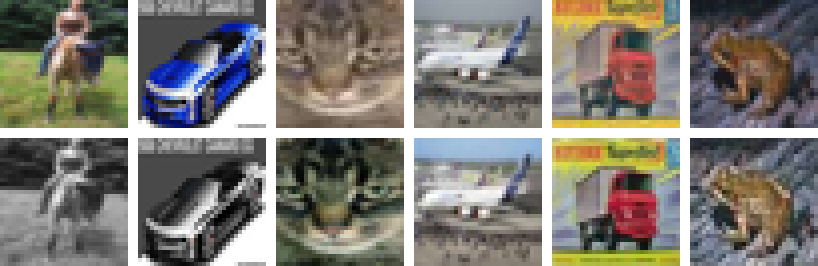
\includegraphics[width=\columnwidth]{cifar_pairs.png}
\caption{Six of the 24 flagged pairs missing from the ciFAIR list. Top: CIFAR-10 test images
9186, 6173, 3572, 4937, 2899, 4413 (all kept in ciFAIR-10). Bottom: their training matches
37082, 4039, 8286, 5994, 27807, 29752. dHash distances 1--4.}\label{fig:pairs}
\end{figure}

The precision at $T{=}4$ is therefore about 96\% (87/91, taking listed pairs as correct), but recall
against ciFAIR is only 22\%: a 64-bit hash of a $32{\times}32$ thumbnail misses crops and
re-shoots that CNN features catch, and raising $T$ trades precision away quickly. The check adds 28\,s to
a cold commit of 60,000 images (7.5\,s to 35.8\,s) and 3\,s to a warm one, since hashes are cached by
content. We see it as a guard that runs on every commit, not a replacement for an embedding search
when a benchmark is built.

\section{Related Work}
\textbf{Leakage.} Kaufman et al.\ formalised leakage in data mining \cite{kaufman2012leakage}, and
Kapoor and Narayanan catalogued it across sciences \cite{kapoor2023leakage}. Audits of visual
benchmarks find duplicates within and across datasets \cite{barz2020cifair,ramos2025leakage,kisel2024flaws,recht2019imagenet},
alongside label errors \cite{northcutt2021labelerrors}; deduplication matters for language models
too \cite{lee2022dedup}. Grouped and blocked cross-validation for structured data is well studied
\cite{roberts2017cv}. These works measure the problem after the fact; we aim to stop it at the point a
dataset version is created.

\textbf{Data validation and versioning.} TFDV \cite{breck2019tfdv} and Deequ \cite{schelter2018deequ}
validate schemas and statistics; mlinspect inspects preprocessing pipelines \cite{grafberger2021mlinspect}.
Deepchecks, mlleak and LeakLens check splits of data frames \cite{deepchecks,mlleak,leaklens}. DVC,
lakeFS and Delta Lake version files or tables \cite{dvc,lakefs,armbrust2020delta}, and datasheets and
Croissant describe datasets \cite{gebru2021datasheets,akhtar2024croissant}. None of them, to our
knowledge, ties group-aware splitting and cross-modal leakage checks to the act of versioning.

\section{Limitations and Next Steps}
The checks are lexical and hash-based: they catch copies, not semantic overlap, and augmentation
detection relies on names and folders. Timings come from a small machine on local disk; object stores
add per-file latency. We have not yet measured how much the leaks we find inflate model scores, nor
audited sensor datasets where subject and recording leakage is common; both are the next experiments.

\bibliographystyle{ACM-Reference-Format}
\bibliography{refs}
\end{document}
